% ---------------------------------------------------------------------------
% DRAFT 3 — Core results: scoring regime (hero) + effective size
% All figures verified against paper/tmlr/NUMBERS.md §3b and §2.
% NOTE: the error-geometry "dissociation index" is deliberately NOT used here
% until scripts/exp8_error_geometry.py has been read and its metric described
% accurately. Do not add it on the strength of its name.
% ---------------------------------------------------------------------------

\section{The Scoring Regime Reorders the Leaderboard}
\label{sec:regime}
\label{sec:budget}

Every model was scored three times over identical predictions. The \textbf{strict} regime is the
four-stage string-matching pipeline of Section~\ref{sec:scoring}. The \textbf{judge-only} regime
takes the verdict of a cross-model judge (phi4-mini, Section~\ref{sec:judge}, sharing no model
family with any of the twelve evaluated systems) as final, in both directions, on every
regulatory-interpretation, numerical-reasoning, and temporal-reasoning prediction---not only the
ones strict scoring marked wrong. The \textbf{judge-augmented} regime instead takes
strict-OR-judge: a strict-correct answer counts even if the judge disputes it, and a strict-wrong
answer counts if the judge accepts it. Strict and judge-only are this paper's two primary regimes;
judge-augmented is an operational sensitivity regime, included because a practitioner who applies a
judge only to rescue strict failures---never to challenge strict successes---is applying exactly
this asymmetric rule, not because we consider it authoritative. Contradiction-detection items use
exact Yes/No matching in all three regimes and need no judge review.

Nothing about the models changed between regimes. Only the rule changed.

\begin{figure}[t]
\centering
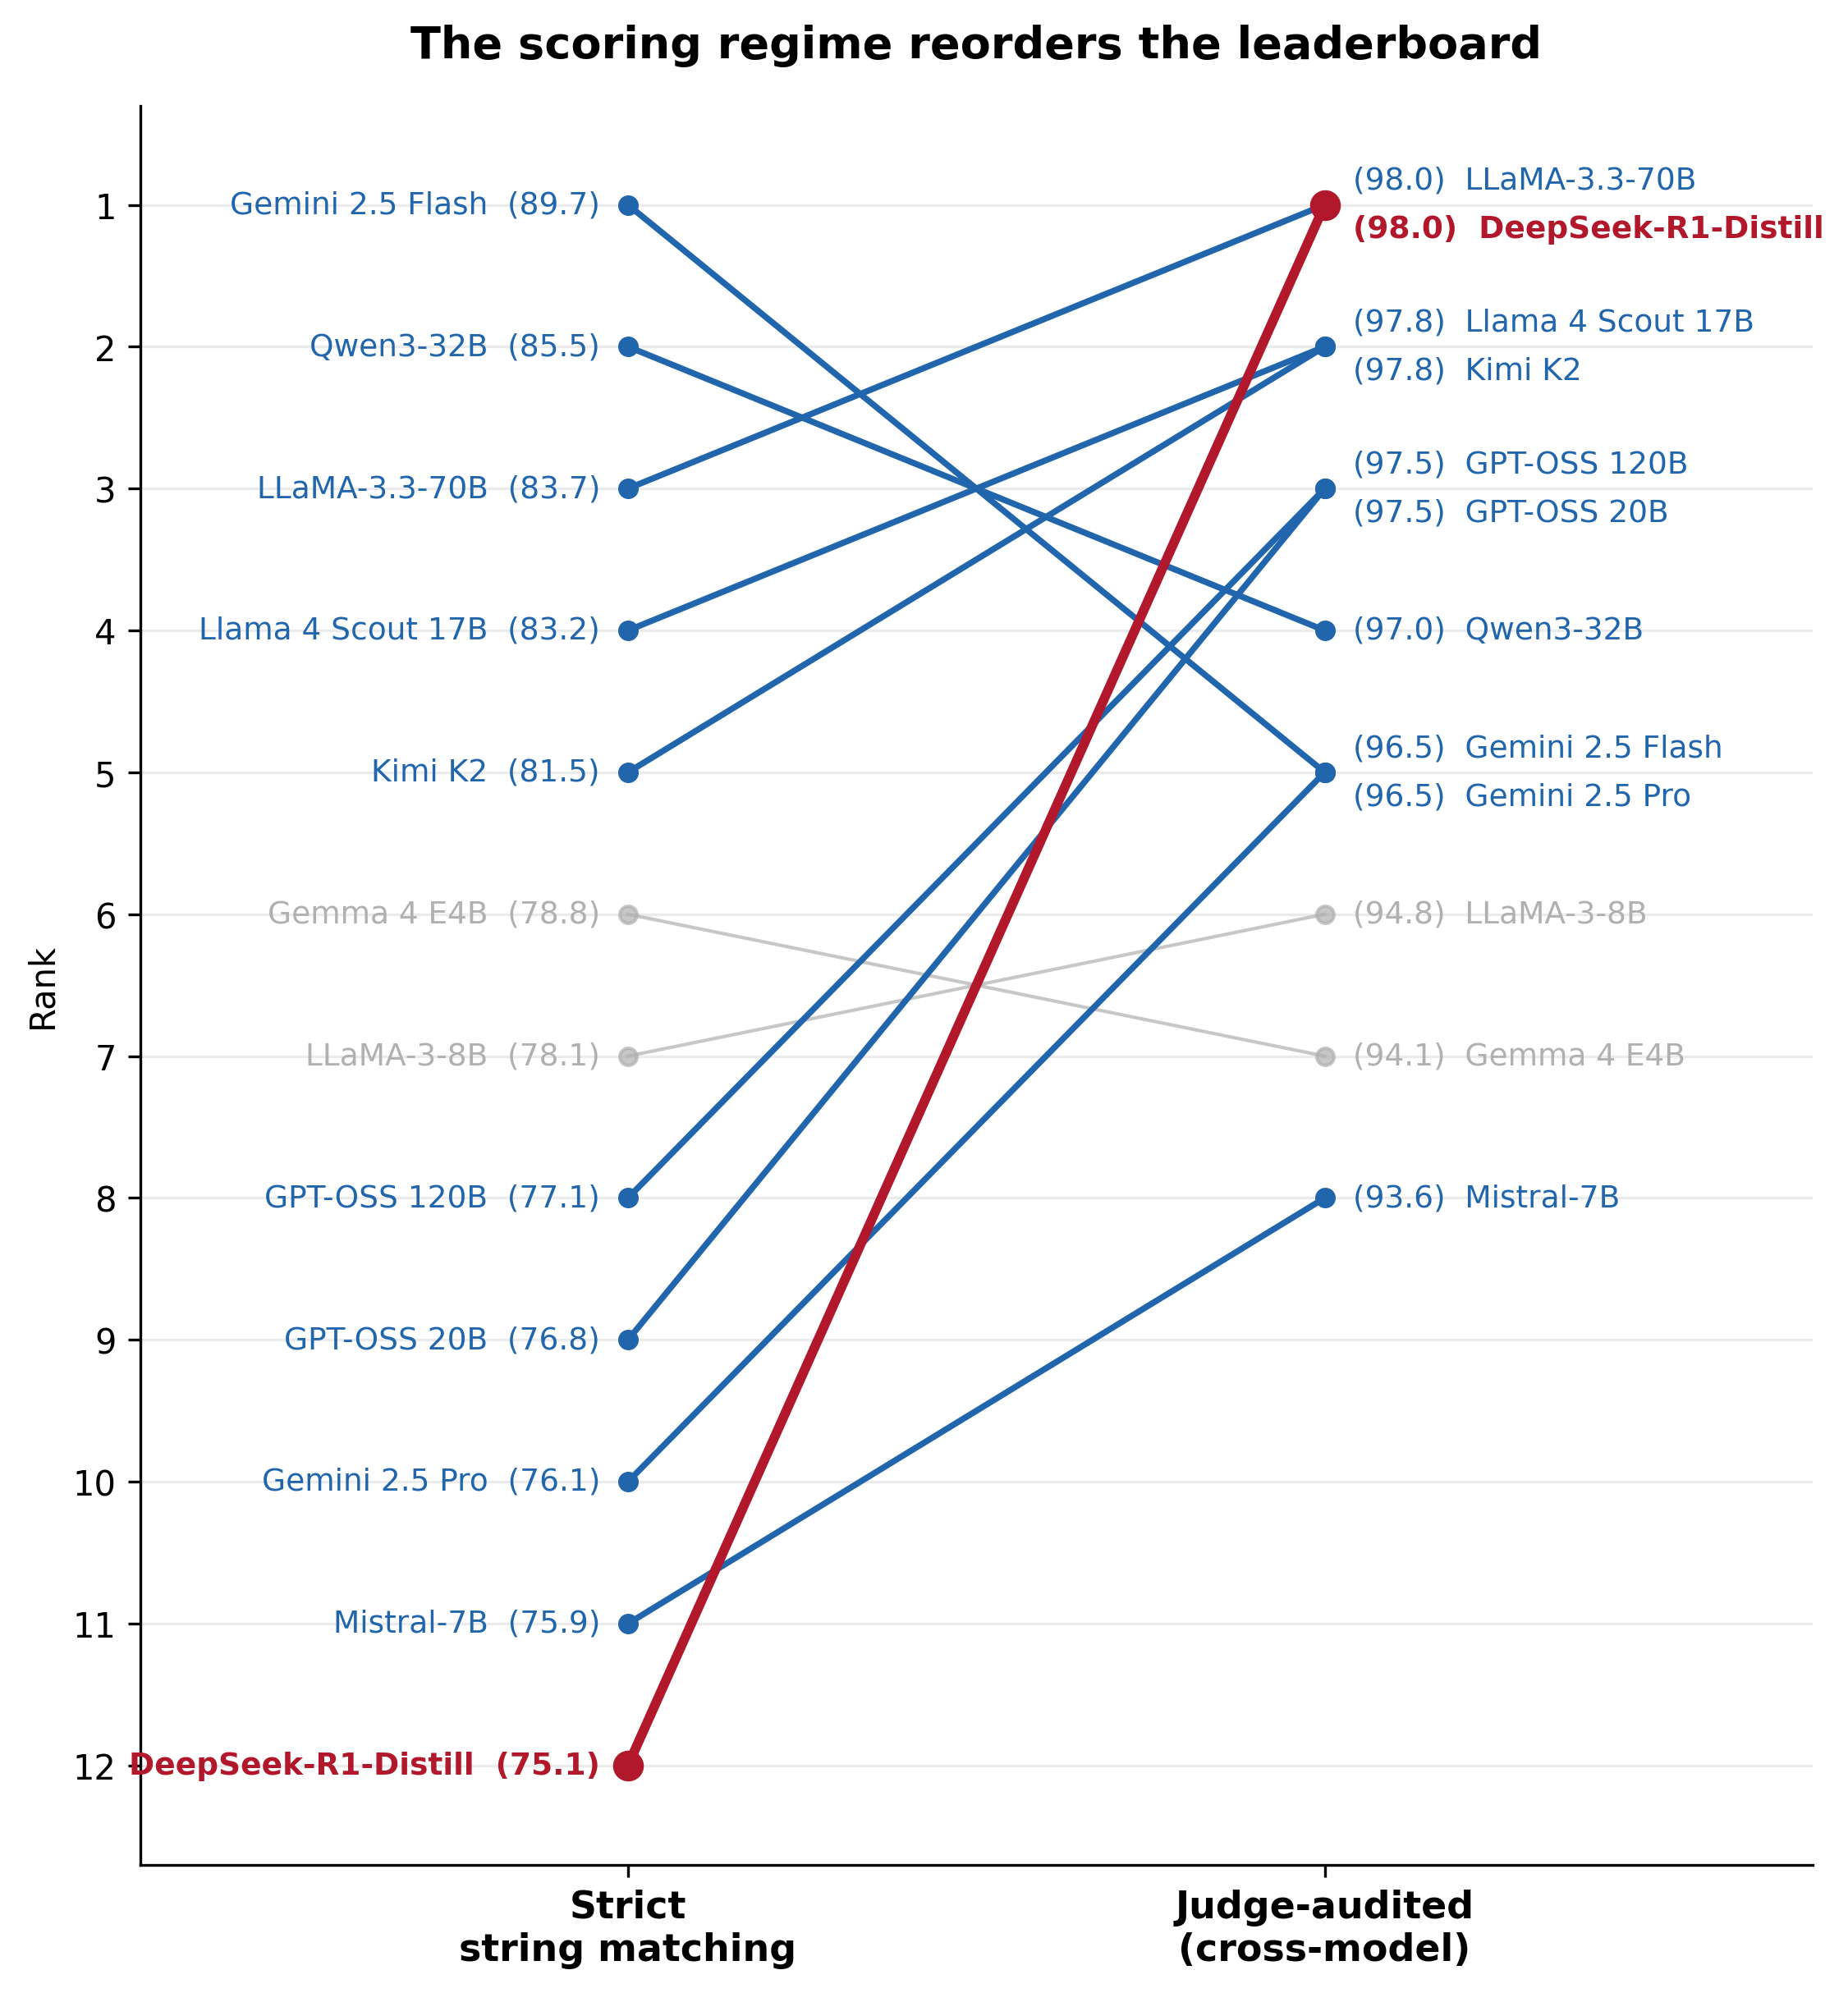
\includegraphics[width=0.95\linewidth]{figures/figure_regime_shift.png}
\caption{Model rank under strict string matching (left), the judge's own verdict (centre), and the
judge-augmented composite (right), over identical predictions. The centre column is this paper's
second primary regime; the right column is a sensitivity regime, shown in a lighter tone. Coloured
lines move by two or more positions between strict and judge-only. Tied scores share a rank.}
\label{fig:regime}
\end{figure}

Appendix~\ref{app:regimetable} tabulates exact accuracy and rank for all twelve models under all
three regimes; the discussion below states the comparisons that matter.

\textbf{Strict and judge-only show no positive rank correspondence.} Strict accuracy spans
75.12--89.66\%; judge-only accuracy spans 87.19--94.83\%, with a different leader (Gemini 2.5 Pro)
and a different trailer (Gemma 3 4B) than strict scoring's (Gemini 2.5 Flash, DeepSeek-R1-Distill).
Across the twelve models, Spearman $\rho = -0.273$ ($p = 0.39$), Kendall $\tau = -0.168$ ($p = 0.45$).
With twelve models these tests have little power, so we do not claim the rankings are negatively
correlated in a strict statistical sense---we claim they show no positive correspondence, which
Figure~\ref{fig:regime} and Appendix~\ref{app:regimetable} show directly: only one of twelve models
(Kimi K2, rank 5 under each) holds the same rank under both. Neither regime is more correct than the other; each answers a different question
(exact reproduction of a reference format, versus a second model's judgment of substantive
correctness), and a benchmark that reports only one has silently chosen which question to answer.

\textbf{The judge-augmented sensitivity regime illustrates how far a single asymmetric choice can
move a model.} Under strict-OR-judge, DeepSeek-R1-Distill---12th of twelve, last place, under
strict scoring---reaches an exact tie for 1st with LLaMA-3.3-70B (both 398/406, 98.0\%). Of its 99
strict errors on REG/NUM/TMP, 93 are reclassified as correct by the cross-model judge---93.9\%---
leaving 6 residual failures, the fewest of any model in the study. Under the judge's own verdict
alone (judge-only, not augmented), DeepSeek-R1-Distill ranks 7th of twelve, tied with Qwen3-32B
(92.4\%): the judge
recovers most of its strict failures but also disputes some of its strict successes, and the
augmented regime's asymmetric rule---rescue but never reject---is what produces the 1st-place tie.
We report this as what it is: a real, measured consequence of one specific, defensible-but-partial
way of combining two scores, not evidence that DeepSeek-R1-Distill's regulatory reasoning is
best-in-field. Its strict score is a measurement under a particular operational
definition---exact and near-exact string match against a reference format---not a direct measurement
of its regulatory reasoning; under that definition its output sits far from the reference, and the
model narrates its working where the system prompt asked for an answer with no preamble. We tested,
rather than assumed, whether output length itself explains which strict failures get reclassified
(Section~\ref{sec:discussion}); it does not survive adjustment for task and model composition, so we
do not claim narration or verbosity as the mechanism---only that the judge and strict scoring
disagree on this model's output more than on any other's, for reasons this paper's evidence does not
fully resolve.

A second effect is visible in the accuracies rather than the ranks. The full field spans 14.5 points
under strict scoring (75.12--89.66) and just 3.9 points under judge-augmented scoring (94.1--98.0);
judge-only compresses it to 7.6 points (87.19--94.83). Compression under either judge-involving
regime is real, but the size of the effect depends on which one: judge-augmented's asymmetric rule
compresses roughly twice as much as judge-only's symmetric one, because it can only ever move scores
upward.

This has a practical reading that is not a criticism of string matching. A compliance workflow that
consumes model output through a format-sensitive parser really would fail on DeepSeek-R1-Distill's
93 reclassified items, and for that deployment question the strict number is the honest one. What
the strict number cannot do is answer which model reasons best about the underlying regulatory
content, and the two questions are routinely reported as if they were the same quantity.

\subsection{Completion Budget as a Confound}
\label{sec:budget-results}

Section~\ref{sec:models} disclosed that the original evaluation used per-model completion budgets
that were not uniform (200--2048 tokens, chosen per provider for cost reasons) and that write-time
logging separately capped stored predictions at 200--500 characters regardless of what the model
generated (Appendix~\ref{app:truncation}). Both are operational choices, not properties of the
models, and both can depress a model's strict score independently of its underlying answer. We
re-ran the 10 of 12 models reachable under current API credentials at a single uniform completion
budget of 512 tokens---selected by pilot (Appendix~\ref{app:matched-budget-ids})---logging the
complete prediction plus provider finish-reason and completion-token count for every item, neither of
which the original release records for any model. Gemini 2.5 Pro is unreachable on any fresh API key;
Gemini 2.5 Flash's re-run is not yet complete (Appendix~\ref{app:matched-budget-ids} gives both
reasons in full).

\begin{table}[t]
\centering\small
\begin{tabular}{lrrrrr}
\toprule
Model & Orig.\ budget & Original & Matched (512) & $\Delta$pp & Trunc.\ @512 \\
\midrule
LLaMA-3-8B & 300 & 78.33 & 82.27 & +3.94 & 0.0\% \\
Mistral-7B & 300 & 75.37 & 77.83 & +2.46 & 0.0\% \\
Gemma 3 4B & 512 & 79.06 & 78.82 & -0.24 & 0.0\% \\
GPT-OSS 120B & 512 & 75.62 & 76.85 & +1.23 & 1.7\% \\
GPT-OSS 20B & 512 & 75.62 & 74.88 & -0.74 & 5.2\% \\
DeepSeek-R1-Distill & 2048 & 74.88 & 85.71 & \textbf{+10.83} & 1.2\% \\
LLaMA-3.3-70B & 200 & 81.03 & 84.73 & +3.70 & 0.2\% \\
Llama 4 Scout 17B & 1024 & 81.53 & 80.79 & -0.74 & 0.0\% \\
Kimi K2 & 512 & 81.53 & 81.28 & -0.25 & 5.9\% \\
Qwen3-32B & 1024 & 84.24 & 83.99 & -0.25 & 0.0\% \\
\bottomrule
\end{tabular}

\caption{Strict accuracy under the original per-model budget versus a uniform 512-token budget, same
four-stage scorer, same items. $\Delta$pp is bolded where $|\Delta| \geq 5$. ``Trunc.\ @512'' is the
fraction of matched-run predictions that hit the 512-token cap (\texttt{finish\_reason=length}).
Original completion budgets and truncation rates: Appendix~\ref{app:truncation}.}
\label{tab:matchedbudget}
\end{table}

This re-run changes two things relative to the original release at once---the completion budget and
the removal of the write-time logging cap---so a per-model $\Delta$ here is their joint effect, not
an isolated budget effect; the two cannot be separated post hoc from released data that never
recorded generation-level truncation in the first place. Nine of the ten models shift by at most
4 points in either direction ($-0.74$ to $+3.94$pp), consistent with a modest, mixed-sign operational
effect on top of measurement noise. DeepSeek-R1-Distill is an outlier at $+10.83$pp; we report it
without endorsing a single explanation, since it does not correlate with each model's original
write-time-cap rate (Pearson $r = 0.09$) and at least one competing explanation, unrelated to budget,
remains live (Appendix~\ref{app:matched-budget-ids} gives both candidates and the evidence for each in
full). What the re-run supports without qualification is the general point: strict accuracy is
sensitive to completion budget and logging configuration, sometimes by several points, for models
whose original budget was well below 512---further evidence, alongside the scoring-regime result,
that a single leaderboard number is a property of the measurement protocol as much as of the model.

\section{Discriminative Coverage: How Many Items Actually Discriminate}
\label{sec:effsize}

A benchmark's nominal size is the number of items it contains. Its \textbf{discriminative
coverage}, for the purpose of separating systems, is the number of items on which systems actually
differ. An item that every model answers correctly contributes to reported accuracy but
distinguishes no pair of models. (We avoid ``effective size'': it invites confusion with
effective-sample-size, a distinct and more specific statistical quantity we do not compute.)

For each item we take $p$, the fraction of the twelve models answering it correctly. The
threshold-light fact is the most robust one: 213 of 406 items (52.5\%) are answered correctly by at
least 11 of the 12 models --- the ceiling category. At $n=12$ models, $p$ only takes values
$k/12$ for integer $k$, and the single achievable value in $(0.9, 1]$ below 1 itself is $11/12
\approx 0.917$; consequently ``$p \ge 0.9$'' and ``$p > 0.90$'' pick out the identical set of items
by construction, not because two independent checks happened to agree. We note this to be precise
about what does and does not constitute corroboration here, not to claim a stronger result than the
arithmetic supports.

\begin{table}[t]
\centering
\caption{Item categories by the fraction of models answering correctly ($p$). Ceiling items are
answered correctly by at least 11 of 12 models; floor items by at most 1 of 12. The discriminative
band is defined by $p$ alone; see the text for why an additional spread threshold on
$s=4p(1-p)$ would not change this category's membership.}
\label{tab:effsize}
\begin{tabular}{lrrl}
\toprule
Category & Items & \% & Criterion \\
\midrule
Ceiling            & 213 & 52.5 & $p \ge 0.9$ \\
Discriminative     & 134 & 33.0 & $0.3 < p < 0.8$ \\
Intermediate       & 52  & 12.8 & remainder \\
Floor              & 7   & 1.7  & $p \le 0.1$ \\
\midrule
Total              & 406 & 100  & \\
\bottomrule
\end{tabular}
\end{table}

The discriminative band in Table~\ref{tab:effsize} is defined by $p$ alone: $0.3 < p < 0.8$, i.e.\
$k \in \{4,\ldots,9\}$ of 12 models correct. An earlier version of this criterion also required
$s=4p(1-p)$ above the sample median; at $n=12$ that second condition never binds within this
$p$-range (its minimum there, at $k=9$, is $s=0.75$, already above the median item's $s=0.306$ at
$k=11$), so it added no information and we removed it rather than retain a criterion that reads as
more selective than it is. 134 items meet the $p$-range criterion.

Half the benchmark sits at ceiling. 213 of 406 items are answered correctly by at least 11 of the
12 models, and 7 more are answered correctly by at most one, so 220 items---slightly over
half---carry almost no information about the relative ordering of these systems. The median item is
answered correctly by 91.7\% of models.

We report this about our own benchmark deliberately. It bears directly on how the results above
should be read: a gap of a few points between two mid-table models rests on a subset of 134 items,
not 406. It also suggests a construction lesson we did not anticipate when building the
benchmark---annotating for coverage of a domain and annotating for discrimination between systems
are different objectives, and expert effort spent on items that every competent model answers
correctly buys descriptive completeness rather than measurement power.

We do not claim this ratio is unusual. We claim it is unmeasured: we are not aware of comparable
benchmarks in this literature that report what fraction of their items separate the systems they
rank, and without that figure a reported accuracy gap cannot be sized against the evidence
supporting it.
